% Created 2021-12-15 Wed 21:03
\documentclass[9pt, b5paper]{article}
\usepackage[UTF8]{ctex}
\usepackage{xltxtra}
\usepackage{bera}
\usepackage[T1]{fontenc}
\usepackage[scaled]{beraserif}
\usepackage[scaled]{berasans}
\usepackage[scaled]{beramono}
\usepackage{graphicx}
\usepackage{xcolor}
\usepackage{multirow}
\usepackage{multicol}
\usepackage{float}
\usepackage{textcomp}
\usepackage{geometry}
\geometry{left=1.2cm,right=1.2cm,top=1.5cm,bottom=1.2cm}
\usepackage{algorithm}
\usepackage{algorithmic}
\usepackage{latexsym}
\usepackage{natbib}
\usepackage{minted}
\newminted{common-lisp}{fontsize=ootnotesize}
\usepackage[xetex,colorlinks=true,CJKbookmarks=true,linkcolor=blue,urlcolor=blue,menucolor=blue]{hyperref}
\author{deepwaterooo}
\date{\today}
\title{Android Service}
\hypersetup{
  pdfkeywords={},
  pdfsubject={},
  pdfcreator={Emacs 27.1 (Org mode 8.2.7c)}}
\begin{document}

\maketitle
\tableofcontents


\section{Android:Service生命周期完全解析}
\label{sec-1}
\begin{itemize}
\item 目录

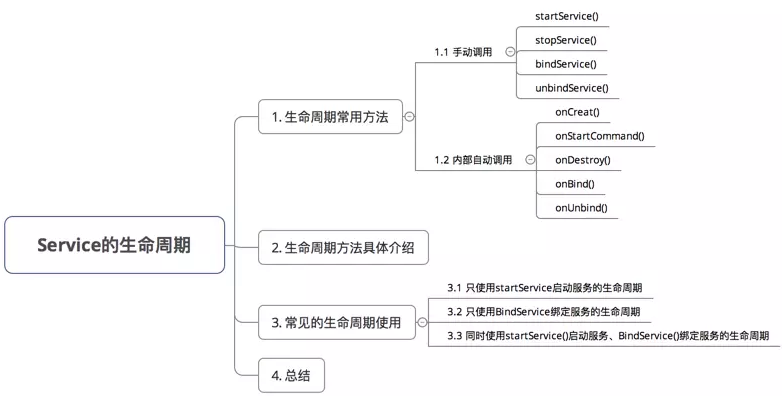
\includegraphics[width=.9\linewidth]{./pic/serviceLifeCycle.png}
\end{itemize}
\subsection{生命周期 常用方法}
\label{sec-1-1}

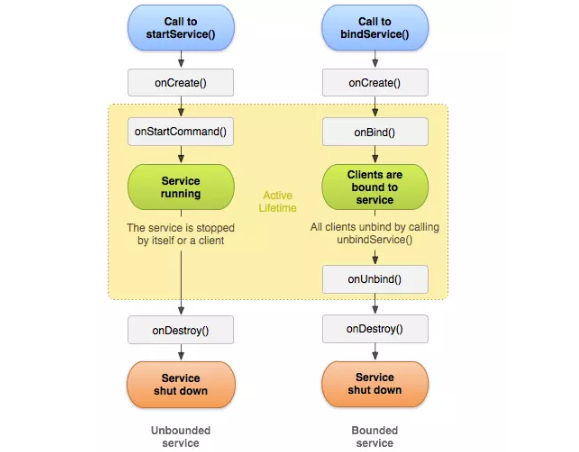
\includegraphics[width=.9\linewidth]{./pic/serviceCallbacks.png}
\begin{itemize}
\item 在Service的生命周期里,常用的有:
\begin{itemize}
\item 4个手动调用的方法
\end{itemize}
\end{itemize}
\begin{center}
\begin{tabular}{ll}
\hline
手动调用方法 & 作用\\
\hline
startService() & 启动服务\\
stopService() & 关闭服务\\
bindService() & 绑定服务\\
unbindService() & 解绑服务\\
\hline
\end{tabular}
\end{center}
\begin{itemize}
\item 5个自动调用的方法
\end{itemize}
\begin{center}
\begin{tabular}{ll}
\hline
内部自动调用的方法 & 作用\\
\hline
onCreate() & 创建服务\\
onStartCommand() & 开始服务\\
onDestroy() & 销毁服务\\
onBind() & 绑定服务\\
onUnbind() & 解绑服务\\
\hline
\end{tabular}
\end{center}
\subsection{startService方式}
\label{sec-1-2}
\begin{itemize}
\item startService()只要一个Intent参数,指定要开启的Service即可
\end{itemize}
\begin{minted}[frame=lines,fontsize=\scriptsize,linenos=false]{java}
Intent intent = new Intent(MainActivity.this, MyService.class);
\end{minted}
\begin{itemize}
\item 当调用Service的startService()后,
\begin{itemize}
\item Service首次启动,则先调用onCreate(),在调用onStartCommand()
\item Service已经启动,则直接调用onStartCommand()
\end{itemize}
\item 当调用stopSelf()或者stopService()后,会执行onDestroy(),代表Service生命周期结束。
\item startService方式启动Service不会调用到onBind()。startService可以多次调用,每次调用都会执行onStartCommand()。不管调用多少次startService,只需要调用一次stopService就结束。如果startService后没有调用stopSelf或者stopService,则Service一直存活并运行在后台。
\item onStartCommand的返回值一共有3种
\end{itemize}
\begin{minted}[frame=lines,fontsize=\scriptsize,linenos=false]{java}
START_STICKY = 1 // service所在进程被kill之后,系统会保留service状态为开始状态。系统尝试重启service,当服务被再次启动,传递过来的intent可能为null,需要注意。
START_NOT_STICKY = 2 // service所在进程被kill之后,系统不再重启服务
START_REDELIVER_INTENT = 3 // 系统自动重启service,并传递之前的intent
\end{minted}
\begin{itemize}
\item 默认返回START\_STICKY;
\end{itemize}
\subsection{bindService方式}
\label{sec-1-3}
\begin{itemize}
\item 通过bindService绑定Service相对startService方式要复杂一点。
\item 由于bindService是异步执行的,所以需要额外构建一个ServiceConnection对象用与接收bindService的状态,同时还要指定bindService的类型。
\end{itemize}
\begin{minted}[frame=lines,fontsize=\scriptsize,linenos=false]{java}
// 1. 定义用于通信的对象,在Service的onBind()中返回的对象。
public class MyBind extends Binder {
    public int mProcessId;
}
// 2. 定义用于接收状体的ServiceConnection
mServiceConnection = new ServiceConnection() {
    @Override
    public void onServiceConnected(ComponentName name, IBinder service) {
        // 和服务绑定成功后,服务会回调该方法
        // 服务异常中断后重启,也会重新调用改方法
        MyService.MyBind myBinder = (MyService.MyBind) service;
    }
    @Override
    public void onNullBinding(ComponentName name) {
        // Service的onBind()返回null时将会调用这个方法,并不会调用onServiceConnected()
    }
    @Override
    public void onServiceDisconnected(ComponentName name) {
        //  当服务异常终止时会调用。
        //  注意,unbindService时不会调用
    }
};
// 3. 在需要的地方绑定到Service
bindService(intent, mServiceConnection, BIND_AUTO_CREATE);
\end{minted}
\begin{itemize}
\item 复制代码bindService()也可以调用多次,与startService()不同,当发起对象与Service已经成功绑定后,不会多次返回ServiceConnection中的回调方法。
\item 通过bindService方式与Service进行绑定后,当没有对象与Service绑定后,Service生命周期结束,这个过程包括绑定对象被销毁,或者主动掉调用unbindService()
\end{itemize}
\subsection{startService和bindService同时开启}
\label{sec-1-4}
\begin{itemize}
\item 当同时调用startService和bindService后,需要分别调用stopService和unbindService,Service才会走onDestroy()
\item 一个Service必须要在既没有和任何Activity关联又处理停止状态的时候才会被销毁。
\end{itemize}
\subsection{IntentService}
\label{sec-1-5}
\begin{itemize}
\item 通过上面的介绍我们知道,通过StartService形式开启Service时,如果不主动调用stopService,Service将在后台一直运行。同时如果我们在Service中执行耗时操作还是引起ANR异常,为了解决这2个问题,IntentService出现了。
\item 当我们需要执行某些一次性、异步的操作时,IntentService能很好的满足这个场景。
\item IntentService相比于普通的Service,在使用时将不再需要实现onStartCommand(),同时需要实现onHandleIntent()。
\item 真正需要我们处理的逻辑就在onHandleIntent()实现,IntentService会内部自动调用stopSelf()关闭自己。
\item 至于防止ANR异常,具体的实现方式其实还是挺简单,就是在内部新建了子线程,并在子线程中内部的Looper来分发事件
\end{itemize}

\subsection{Service实现IPC通信的2中方式}
\label{sec-1-6}
\subsubsection{借助AIDL实现IPC通信}
\label{sec-1-6-1}
\begin{enumerate}
\item 与远端进程的Service绑定
\label{sec-1-6-1-1}
\begin{itemize}
\item AIDL:Android Interface Definition Language,即Android接口定义语言。
\item Service跨进程传递数据需要借助aidl,主要步骤是这样的:
\begin{itemize}
\item 编写aidl文件,AS自动生成的java类实现IPC通信的代理
\item 继承自己的aidl类,实现里面的方法
\item 在onBind()中返回我们的实现类,暴露给外界
\item 需要跟Service通信的对象通过bindService与Service绑定,并在ServiceConnection接收数据。
\end{itemize}
\item 我们通过代码来实现一下:
\begin{itemize}
\item 首先我们需要新建一个Service
\end{itemize}
\end{itemize}
\begin{minted}[frame=lines,fontsize=\scriptsize,linenos=false]{java}
public class MyRemoteService extends Service {
	@Nullable
        @Override
        public IBinder onBind(Intent intent) {
  		Log.e("MyRemoteService", "MyRemoteService thread id = " + Thread.currentThread().getId());
        return null;
	}
}
\end{minted}
\begin{itemize}
\item 在manifest文件中声明我们的Service同时指定运行的进程名, \uline{这里并是不只能写remote进程名,你想要进程名都可以}
\end{itemize}
\begin{minted}[frame=lines,fontsize=\scriptsize,linenos=false]{xml}
<service
        android:name=".service.MyRemoteService"
        android:process=":remote" />
\end{minted}
\begin{itemize}
\item 新建一个aidl文件用户进程间传递数据。
\begin{itemize}
\item AIDL支持的类型:八大基本数据类型、String类型、CharSequence、List、Map、自定义类型。List、Map、自定义类型放到下文讲解。
\item Android Studio--> new--> AIDL --> AIDL file 里面会有一个默认的实现方法,删除即可,这里我们新建的文件如下:
\end{itemize}
\end{itemize}
\begin{minted}[frame=lines,fontsize=\scriptsize,linenos=false]{java}
package xxxx;// aidl所在的包名
interface IProcessInfo { // interface之前不能有修饰符
	// 你想要的通信用的方法都可以在这里添加
	int getProcessId();
}
\end{minted}
\begin{itemize}
\item 实现我们的aidl类
\end{itemize}
\begin{minted}[frame=lines,fontsize=\scriptsize,linenos=false]{java}
public class IProcessInfoImpl extends IProcessInfo.Stub { // IProcessInfo.Stub
	@Override
	public int getProcessId() throws RemoteException {
  		return android.os.Process.myPid();
	}
}
\end{minted}
\begin{itemize}
\item 在Service的onBind()中返回
\end{itemize}
\begin{minted}[frame=lines,fontsize=\scriptsize,linenos=false]{java}
public class MyRemoteService extends Service {
	IProcessInfoImpl mProcessInfo = new IProcessInfoImpl();
	@Nullable
	@Override
	public IBinder onBind(Intent intent) {
  		Log.e("MyRemoteService", "MyRemoteService thread id = " + Thread.currentThread().getId());
        return mProcessInfo;
	}
}
\end{minted}
\begin{itemize}
\item 绑定Service
\end{itemize}
\begin{minted}[frame=lines,fontsize=\scriptsize,linenos=false]{java}
mTvRemoteBind.setOnClickListener(new View.OnClickListener() {
        @Override public void onClick(View v) {
            Intent intent = new Intent(MainActivity.this, MyRemoteService.class);
            bindService(intent, mRemoteServiceConnection, BIND_AUTO_CREATE);
        }
    });
mRemoteServiceConnection = new ServiceConnection() {
    @Override
    public void onServiceConnected(ComponentName name, IBinder service) {
        Log.e("MainActivity", "MyRemoteService onServiceConnected");
        IProcessInfo processInfo = IProcessInfo.Stub.asInterface(service); // 通过aidl取出数据
        try {
            Log.e("MainActivity", "MyRemoteService process id = " + processInfo.getProcessId());
        } catch (RemoteException e) {
            e.printStackTrace();
        }
    }
    @Override
    public void onServiceDisconnected(ComponentName name) {
        Log.e("MainActivity", "MyRemoteService onServiceDisconnected");
    }
};
\end{minted}
\begin{itemize}
\item 只要绑定成功就能在有log打印成MyRemoteService所在进程的进程id。这样我们就完成了跟不同进程的Service通信的过程。
\end{itemize}
\item 调用其他app的Service
\label{sec-1-6-1-2}
\begin{itemize}
\item 跟调同app下不同进程下的Service相比,调用其他的app定义的Service有一些细微的差别
\end{itemize}
\begin{enumerate}
\item 由于需要其他app访问,所以之前的bindService()使用的隐式调用不再合适,需要在Service定义时定义action
\label{sec-1-6-1-2-1}
\begin{itemize}
\item 我们在定义的线程的App A 中定义如下Service:
\end{itemize}
\begin{minted}[frame=lines,fontsize=\scriptsize,linenos=false]{xml}
<service android:name=".service.ServerService">
  <intent-filter>
	<!-- 这里的action需要自定义 -->
    <action android:name="com.jxx.server.service.bind" />
    <category android:name="android.intent.category.DEFAULT" />
  </intent-filter>
</service>
\end{minted}
\item 我们在需要bindService的App B 中需要做这些处理
\label{sec-1-6-1-2-2}
\begin{itemize}
\item 首先要将A中定义的aidl文件复制到B中,比如我们在上面定义的IProcessInfo.aidl这个文件,包括路径在内需要原封不动的复制过来。
\item 在B中调用Service通过显式调用
\end{itemize}
\begin{minted}[frame=lines,fontsize=\scriptsize,linenos=false]{java}
mTvServerBind.setOnClickListener(new View.OnClickListener() {
    @Override
    public void onClick(View v) {
        Intent intent = new Intent();
        intent.setAction("com.jxx.server.service.bind"); // Service的action
        intent.setPackage("com.jxx.server"); // App A 的包名
        bindService(intent, mServerServiceConnection, BIND_AUTO_CREATE);
    }
});
\end{minted}
\end{enumerate}
\item aidl中自定义对象的传递
\label{sec-1-6-1-3}
\begin{itemize}
\item 主要步骤如下:
\begin{itemize}
\item 定义自定对象,需要实现Parcelable接口
\item 新建自定义对象的aidl文件
\item 在传递数据的aidl文件中引用自定义对象
\item 将自定义对象以及aidl文件拷贝到需要bindService的app中,主要路径也要原封不动
\end{itemize}
\item 我们来看一下具体的代码:
\end{itemize}
\begin{enumerate}
\item 定义自定义对象,并实现Parcelable接口
\label{sec-1-6-1-3-1}
\begin{minted}[frame=lines,fontsize=\scriptsize,linenos=false]{java}
public class ServerInfo implements Parcelable {
    String mPackageName;

    public ServerInfo() { }
    public String getPackageName() {
        return mPackageName;
    }
    public void setPackageName(String packageName) {
        mPackageName = packageName;
    }
    protected ServerInfo(Parcel in) {
        mPackageName = in.readString();
    }
    public static final Creator<ServerInfo> CREATOR = new Creator<ServerInfo>() {
        @Override
        public ServerInfo createFromParcel(Parcel in) {
            return new ServerInfo(in);
        }
        @Override
        public ServerInfo[] newArray(int size) {
            return new ServerInfo[size];
        }
    };
    @Override
        public int describeContents() {
        return 0;
    }
    @Override
        public void writeToParcel(Parcel dest, int flags) {
        dest.writeString(mPackageName);
    }
// 使用out或者inout修饰时需要自己添加这个方法
    public void readFromParcel(Parcel dest) {
        mPackageName = dest.readString();
    }
}
\end{minted}
\item 新建自定义对象的aidl文件
\label{sec-1-6-1-3-2}
\begin{minted}[frame=lines,fontsize=\scriptsize,linenos=false]{java}
package com.jxx.server.aidl;
// 注意parcelable 是小写的
parcelable ServerInfo;
\end{minted}
\item 引用自定义对象
\label{sec-1-6-1-3-3}
\begin{minted}[frame=lines,fontsize=\scriptsize,linenos=false]{java}
package com.jxx.server.aidl;
//就算在同一包下,这里也要导包
import com.jxx.server.aidl.ServerInfo;
interface IServerServiceInfo {
	ServerInfo getServerInfo();
	void setServerInfo(inout ServerInfo serverinfo);
}
\end{minted}
\begin{itemize}
\item 注意这里的set方法,这里用了inout,一共有3种修饰符
\begin{itemize}
\item in:客户端写入,服务端的修改不会通知到客户端
\item out:服务端修改同步到客户端,但是服务端获取到的对象可能为空
\item inout:修改都是同步的
\end{itemize}
\item 当使用out和inout时,除了要实现Parcelable外还要手动添加readFromParcel(Parcel dest)
\end{itemize}
\item 拷贝自定义对象以及aidl文件到在要引用的App中即可。
\label{sec-1-6-1-3-4}
\item 引用
\label{sec-1-6-1-3-5}
\begin{minted}[frame=lines,fontsize=\scriptsize,linenos=false]{java}
mServerServiceConnection = new ServiceConnection() {
        @Override
        public void onServiceConnected(ComponentName name, IBinder service) {
            IServerServiceInfo serverServiceInfo = IServerServiceInfo.Stub.asInterface(service);
            try {
                ServerInfo serviceInfo = serverServiceInfo.getServerInfo();
                Log.e("MainActivity", "ServerService packageName = " + serviceInfo.getPackageName());
            } catch (RemoteException e) {
                e.printStackTrace();
            }
        }

        @Override
        public void onServiceDisconnected(ComponentName name) {
            Log.e("MainActivity", "ServerService onServiceDisconnected");
        }
    };
\end{minted}
\begin{itemize}
\item List、Map中引用的对象也应该是符合上面要求的自定义对象,或者其他的几种数据类型。
\end{itemize}
\end{enumerate}
\end{enumerate}
\subsubsection{使用Messenger实现IPC通信}
\label{sec-1-6-2}
\begin{itemize}
\item 步骤是这样的:
\begin{itemize}
\item 在Server端新建一个Messenger对象,用于响应Client端的注册操作,并在onBind()中传递出去
\item 在Client端的ServiceConnection中,将Server端传递过来的Messenger对象进行保存
\item 同时Client端也新建一个Messenger对象,通过Server传递过来的Messenger注册到Server端,保持通信用。
\item 不管是否进行unbindService()操作,只要Client保有Server端的Messenger对象,仍然能和Server端进行通信。
\end{itemize}
\end{itemize}
\begin{enumerate}
\item Server端代码
\label{sec-1-6-2-1}
\begin{minted}[frame=lines,fontsize=\scriptsize,linenos=false]{java}
public class MessengerService extends Service {
    static final int MSG_REGISTER_CLIENT = 1;
    static final int MSG_UNREGISTER_CLIENT = 2;
    static final int MSG_SET_VALUE = 3;
    // 这个是给client端接收参数用的
    static final int MSG_CLIENT_SET_VALUE = 4;

    private Messenger mMessenger = new Messenger(new ServiceHandler());

    static class ServiceHandler extends Handler {
        private final List<Messenger> mMessengerList = new ArrayList<>();
        @Override public void handleMessage(Message msg) {
            switch (msg.what) {
            case MSG_REGISTER_CLIENT:
                mMessengerList.add(msg.replyTo);
                break;
            case MSG_UNREGISTER_CLIENT:
                mMessengerList.remove(msg.replyTo);
                break;
            case MSG_SET_VALUE:
                int value = msg.arg1;
                for (Messenger messenger : mMessengerList) 
                    try {
                        messenger.send(Message.obtain(null, MSG_CLIENT_SET_VALUE, value, 0));
                    } catch (RemoteException e) {
                        e.printStackTrace();
                    }
                break;
            default:
                super.handleMessage(msg);
            }
        }
    }
    @Nullable @Override public IBinder onBind(Intent intent) {
        return mMessenger.getBinder();
    }
}
\end{minted}
\item Client端代码
\label{sec-1-6-2-2}
\begin{minted}[frame=lines,fontsize=\scriptsize,linenos=false]{java}
public class MessengerClientActivity extends AppCompatActivity {
    // 这些类型要和Server端相对应
    static final int MSG_REGISTER_CLIENT = 1;
    static final int MSG_UNREGISTER_CLIENT = 2;
    static final int MSG_SET_VALUE = 3;
    static final int MSG_CLIENT_SET_VALUE = 4;

    class ClientHandler extends Handler {
        @Override public void handleMessage(Message msg) {
            if (msg.what == MSG_CLIENT_SET_VALUE) {
                mTvValue.setText(msg.arg1 + "");
            } else {
                super.handleMessage(msg);
            }
        }
    }
    TextView mTvServerBind;
    TextView mTvServerUnbind;
    TextView mTvValue;
    TextView mTvSend;

    ServiceConnection mServerServiceConnection;
    Messenger mServerMessenger;

    @Override
        protected void onCreate(@Nullable Bundle savedInstanceState) {
        super.onCreate(savedInstanceState);
        setContentView(R.layout.activity_messenger);

        mTvServerBind = findViewById(R.id.tv_server_bind);
        mTvServerUnbind = findViewById(R.id.tv_server_unbind);
        mTvValue = findViewById(R.id.tv_value);
        mTvSend = findViewById(R.id.tv_send);

        mTvServerBind.setOnClickListener(new View.OnClickListener() {
                @Override public void onClick(View v) {
                    Intent intent = new Intent();
                    intent.setAction("jxx.com.server.service.messenger");
                    intent.setPackage("jxx.com.server");
                    bindService(intent, mServerServiceConnection, BIND_AUTO_CREATE);
                }
            });
        mTvServerUnbind.setOnClickListener(new View.OnClickListener() {
                @Override public void onClick(View v) {
                    // 就算这里我们unbindService,只要我们还保留有mServerMessenger对象,
                    // 我们就能继续与Server通信
                    unbindService(mServerServiceConnection);
                }
            });
        mTvSend.setOnClickListener(new View.OnClickListener() {
                @Override public void onClick(View v) {
                    if (mServerMessenger != null) {
                        try {
                            // 测试一下能否设置数据
                            Message test = Message.obtain(null, MSG_SET_VALUE, new Random().nextInt(100), 0);
                            mServerMessenger.send(test);
                        } catch (RemoteException e) {
                            e.printStackTrace();
                        }
                    }
                }
            });
        mServerServiceConnection = new ServiceConnection() {
            @Override public void onServiceConnected(ComponentName name, IBinder service) {
                // 服务端的messenger
                mServerMessenger = new Messenger(service);
                // 现在开始构client用来传递和接收消息的messenger
                Messenger clientMessenger = new Messenger(new ClientHandler());
                try {
                    // 将client注册到server端
                    Message register = Message.obtain(null, MSG_REGISTER_CLIENT);
                    register.replyTo = clientMessenger; // 这是注册的操作,我们可以在上面的Server代码看到这个对象被取出
                    mServerMessenger.send(register);
                    Toast.makeText(MessengerClientActivity.this, "绑定成功", Toast.LENGTH_SHORT).show();
                } catch (RemoteException e) {
                    e.printStackTrace();
                }
            }

        }
        @Override public void onServiceDisconnected(ComponentName name) {
        }
    }
}
\end{minted}
\end{enumerate}

\section{Android 四大组件:一份全面 \& 简洁的 Service 知识讲解攻略: 太简单,需要总结再相对深一点儿}
\label{sec-2}
\begin{itemize}
\item \url{https://www.jianshu.com/p/d963c55c3ab9}
\end{itemize}
\subsection{前言}
\label{sec-2-1}
Service作为 Android四大组件之一,应用非常广泛
本文将提供一份全面 \& 简洁的 Service知识讲解攻略,希望你们会喜欢
\subsection{目录}
\label{sec-2-2}

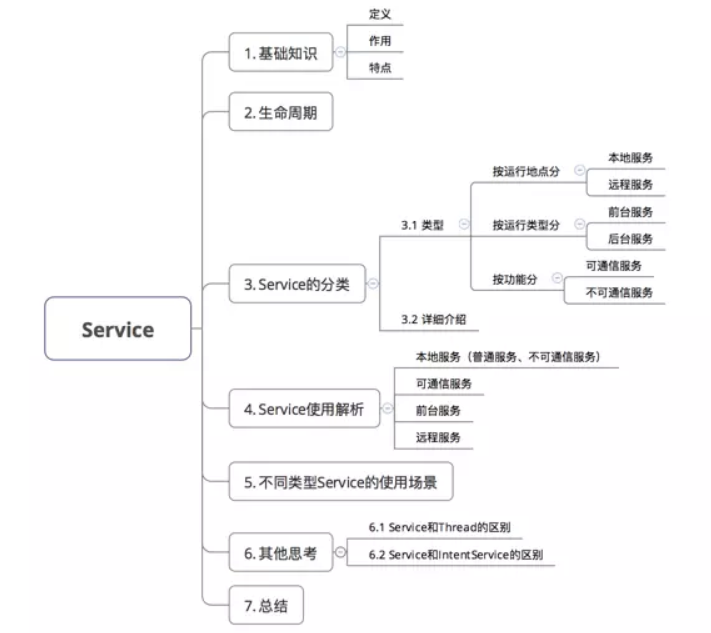
\includegraphics[width=.9\linewidth]{./pic/service.png}
\subsection{简介}
\label{sec-2-3}
\begin{itemize}
\item 定义:服务,是Android四大组件之一, 属于 \textbf{计算型组件}
\item 作用:提供 需在后台长期运行的服务
\begin{itemize}
\item 如:复杂计算、音乐播放、下载等
\end{itemize}
\item 特点:无用户界面、在后台运行、生命周期长
\end{itemize}
\subsection{生命周期}
\label{sec-2-4}
\begin{itemize}
\item 具体请看前一章文章:Android:Service生命周期最全面解析
\begin{itemize}
\item \url{https://www.jianshu.com/p/8d0cde35eb10}
\end{itemize}
\end{itemize}
\subsection{类型}
\label{sec-2-5}
\begin{itemize}
\item Service可按照运行地点、运行类型 \& 功能进行分类,具体如下
\end{itemize}
\subsubsection{具体分类}
\label{sec-2-5-1}
\begin{itemize}
\item 按运行地点分类
\begin{itemize}
\item 本地服务
\item 远程服务
\end{itemize}
\item 按运行类型分类
\begin{itemize}
\item 前台服务
\item 后台服务
\end{itemize}
\item 按功能分类
\begin{itemize}
\item 可通信服务
\item 不可通信服务
\end{itemize}
\end{itemize}
\subsubsection{详细介绍}
\label{sec-2-5-2}
\begin{itemize}
\item 按运行地点分类
\end{itemize}
\begin{center}
\begin{tabular}{lllll}
\hline
类型 & 特点 & 优点 & 缺点 & 应用场景\\
\hline
本地 & -运行在主线程 & -节约资源 & -限制性大 & -需依附某个进程的服务\\
 & -主进程被禁止后,服务也会终止 & -通信方便: & 主进程被禁止后, & (最常用的服务类型如音乐播放)\\
 &  & 因在同一进程因此不需IPC和AIDL & 服务也会终止 & \\
\hline
远程 & -运行在独立进程 & -灵活: & -消耗资源:单独进程 & -系统级别服务\\
 & -服务常驻在后台, & 服务常驻在后台, & -使用AIDL进行IPC复杂 & \\
 & 不受其它activity影响 & 不受其它activity影响 &  & \\
\hline
\end{tabular}
\end{center}

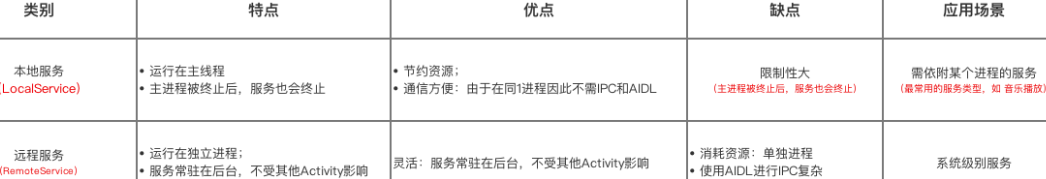
\includegraphics[width=.9\linewidth]{./pic/location.png}
\begin{itemize}
\item 按运行类型分类

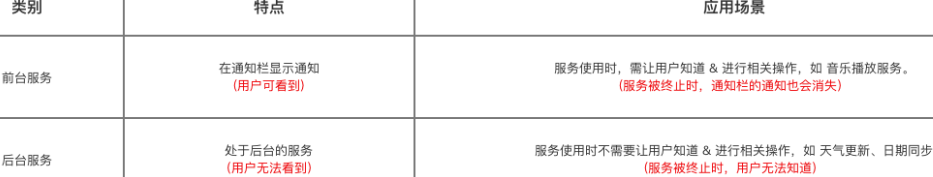
\includegraphics[width=.9\linewidth]{./pic/category.png}
\end{itemize}
\begin{center}
\begin{tabular}{lll}
\hline
类型 & 特点 & 应用场景\\
\hline
前台服务 & - 在通知栏显示通知 & 服务使用时需让用户知道并进行相关操作,如音乐播放\\
 & (用户可看到) & (服务被终止时,通知栏的通知也会消失)\\
\hline
后台服务 & - 处于后台的服务 & 服务使用时不需让用户知道并进行相关操作,如天气更新、日期同步\\
 & (用户无法看到) & (服务被终止时,用户无法知道)\\
\hline
\end{tabular}
\end{center}
\begin{itemize}
\item 按功能分类

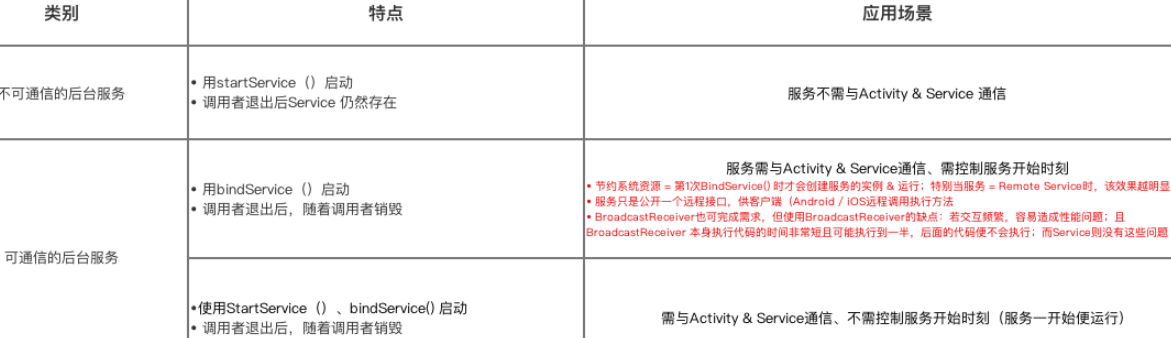
\includegraphics[width=.9\linewidth]{./pic/function.png}
\end{itemize}
\begin{center}
\begin{tabular}{lll}
\hline
类型 & 特点 & 应用场景\\
\hline
不可通信 & -用startService()启动 & 服务不需与Activity \& Service通信\\
后台服务 & -调用者退出后service仍然存在 & \\
 &  & \\
\hline
可通信 & -用bindService()启动 & 服务需与Activity \& Service通信\\
后台服务 & -调用者退出后,随着调用者销毁 & 需控制服务开启时刻\\
 &  & *备注\\
\hline
可通信 & -使用startService()、bindService()启动 & 需与Activity \& Service通信\\
后台服务 & -调用者退出后,随着调用者销毁 & 不需控制服务开启时刻\\
 &  & 服务一开始便运行\\
\hline
\end{tabular}
\end{center}
\begin{itemize}
\item 备注
\begin{itemize}
\item 节约系统资源 = 第一次bindService()时才会创建服务的实例\&运行;特别当服务=remote service时,该效果越明显
\item 服务只是公开一个远程接口,供客户端Android/iOS远程调用执行方法
\item BroadcastReceiver也可完成需求,但使用BroadcastReceiver的缺点:若交互频繁,容易造成性能问题;且BroadcastReceiver本身执行代码的时间非常短且可能执行到一半,后面的代码便不会执行;而Service则没有这些问题
\end{itemize}
\end{itemize}
\subsection{使用讲解}
\label{sec-2-6}
\begin{itemize}
\item 下面,我将介绍每种Service的具体使用
\item 具体请看文章:Android:(本地、可通信的、前台、远程)Service使用全面介绍
\begin{itemize}
\item \url{https://www.jianshu.com/p/e04c4239b07e}
\end{itemize}
\end{itemize}
\subsection{其他思考}
\label{sec-2-7}
\subsubsection{Service 与 Thread的区别}
\label{sec-2-7-1}
\begin{itemize}
\item 结论:Service 与 Thread 无任何关系
\item 之所以有不少人会把它们联系起来,主要因为Service的后台概念
\begin{itemize}
\item \textbf{后台} :后台任务运行完全不依赖UI,即使Activity被销毁 / 程序被关闭,只要进程还在,后台任务就可继续运行
\end{itemize}
\item 关于二者的异同,具体如下图:

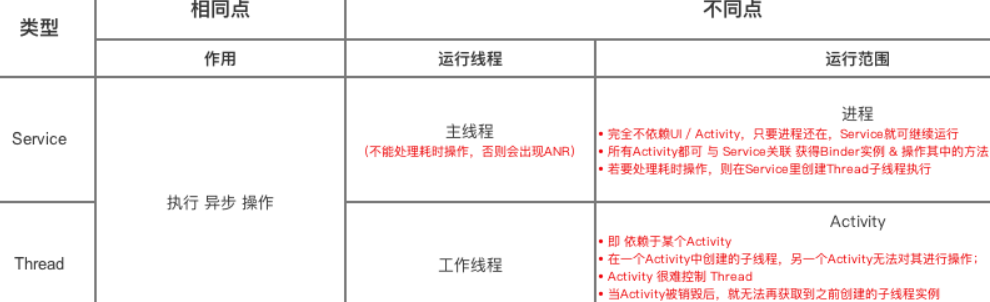
\includegraphics[width=.9\linewidth]{./pic/serviceThreadDiff.png}

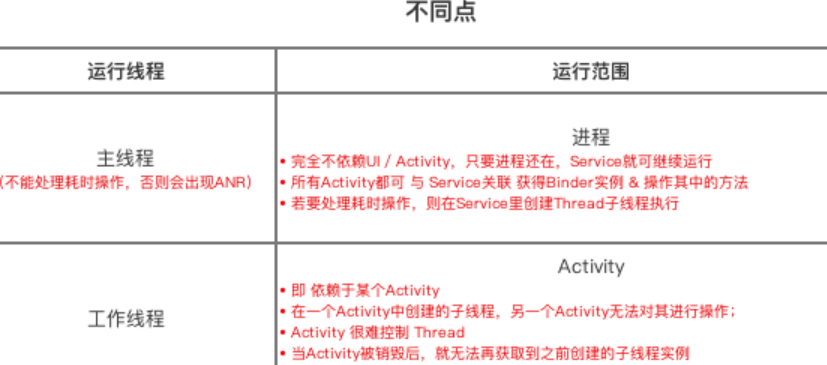
\includegraphics[width=.9\linewidth]{./pic/diff.png}
\item 注:一般会将 Service 和 Thread联合着用,即在Service中再创建一个子线程(工作线程)去处理耗时操作逻辑,如下代码:
\begin{minted}[frame=lines,fontsize=\scriptsize,linenos=false]{java}
@Override  
public int onStartCommand(Intent intent, int flags, int startId) {  
    // 新建工作线程
    new Thread(new Runnable() {  
        @Override  
        public void run() {  
            // 开始执行后台任务  
        }  
    }).start();  
    return super.onStartCommand(intent, flags, startId);  
}  
class MyBinder extends Binder {  
    public void service_connect_Activity() {  
        // 新建工作线程
        new Thread(new Runnable() {  
            @Override  
            public void run() {  
                // 执行具体的下载任务  
            }  
        }).start();  
    }  
}
\end{minted}
\end{itemize}

\subsubsection{Service和IntentService的区别}
\label{sec-2-7-2}
具体请看文章:Android多线程:IntentService用法\&源码
\begin{itemize}
\item \url{https://www.jianshu.com/p/8a3c44a9173a} Android 多线程 解析:IntentService(含源码解析)
\end{itemize}

\section{Android:(本地、可通信的、前台、远程)Service使用全面介绍}
\label{sec-3}
\begin{itemize}
\item \url{https://www.jianshu.com/p/e04c4239b07e}
\end{itemize}
\subsection{前言}
\label{sec-3-1}
Service作为Android四大组件之一,应用非常广泛
本文将介绍Service最基础的知识:Service的生命周期
如果你对Service还未了解,建议先阅读我写的文章:
Android四大组件:Service史上最全面解析
\subsection{目录}
\label{sec-3-2}

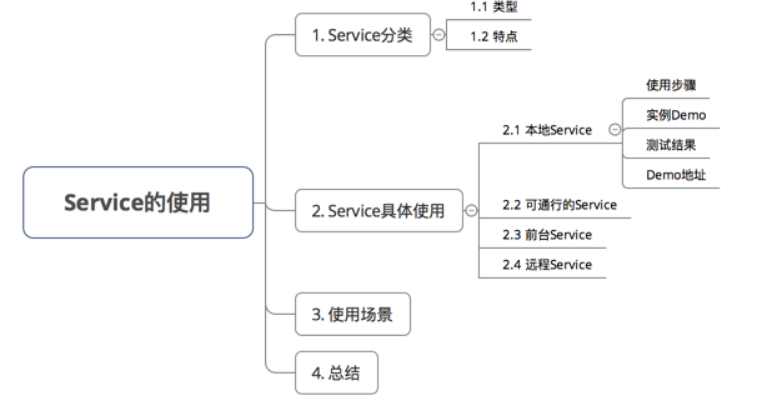
\includegraphics[width=.9\linewidth]{./pic/service2.png}
\subsection{Service分类}
\label{sec-3-3}
\subsubsection{Service的类型}
\label{sec-3-3-1}
\begin{itemize}
\item 按运行地点分类
\begin{itemize}
\item 本地服务
\item 远程服务
\end{itemize}
\item 按运行类型分类
\begin{itemize}
\item 前台服务
\item 后台服务
\end{itemize}
\item 按功能分类
\begin{itemize}
\item 可通信服务
\item 不可通信服务
\end{itemize}
\end{itemize}
\subsubsection{特点}
\label{sec-3-3-2}
\begin{itemize}
\item 详见前一章的三个表格
\end{itemize}
\subsection{具体使用解析}
\label{sec-3-4}
\subsubsection{本地Service}
\label{sec-3-4-1}
\begin{itemize}
\item 这是最普通、最常用的后台服务Service。
\end{itemize}
\begin{enumerate}
\item 使用步骤
\label{sec-3-4-1-1}
\begin{itemize}
\item 步骤1:新建子类继承Service类
\begin{itemize}
\item 需重写父类的 onCreate()、onStartCommand()、onDestroy()和onBind()方法
\end{itemize}
\item 步骤2:构建用于启动Service的Intent对象
\item 步骤3:调用startService()启动Service、调用stopService()停止服务
\item 步骤4:在AndroidManifest.xml里注册Service
\end{itemize}
\item 实例Demo
\label{sec-3-4-1-2}
接下来我将用一个实例Demo进行本地Service说明
\begin{itemize}
\item 建议先下载Demo再进行阅读:(carson.ho的Github地址)Demo\_for\_Service
\begin{itemize}
\item \url{https://github.com/Carson-Ho/Demo_Service/tree/5e2a70cf2d75c56bbfa1abc0ead16c5ad8cae83f}
\end{itemize}
\item 步骤1:新建子类继承Service类
\begin{itemize}
\item 需重写父类的onCreate()、onStartCommand()、onDestroy()和onBind()
\item MyService.java
\end{itemize}
\begin{minted}[frame=lines,fontsize=\scriptsize,linenos=false]{java}
public class MyService extends Service {
    // 启动Service之后,
    // 就可以在onCreate()或onStartCommand()方法里去执行一些具体的逻辑
    // 由于这里作Demo用,所以只打印一些语句
    @Override
    public void onCreate() {
        super.onCreate();
        System.out.println("执行了onCreat()");
    }
    @Override
    public int onStartCommand(Intent intent, int flags, int startId) {
        System.out.println("执行了onStartCommand()");
        return super.onStartCommand(intent, flags, startId);
    }
    @Override
    public void onDestroy() {
        super.onDestroy();
        System.out.println("执行了onDestory()");
    }
    @Nullable
    @Override
    public IBinder onBind(Intent intent) {
        return null;
    }
}
\end{minted}
\item 步骤2:在主布局文件设置两个Button分别用于启动和停止Service
\begin{itemize}
\item activity\_main.xml
\end{itemize}
\begin{minted}[frame=lines,fontsize=\scriptsize,linenos=false]{xml}
<?xml version="1.0" encoding="utf-8"?>
<RelativeLayout xmlns:android="http://schemas.android.com/apk/res/android"
    xmlns:tools="http://schemas.android.com/tools"
    android:layout_width="match_parent"
    android:layout_height="match_parent"
    android:paddingBottom="@dimen/activity_vertical_margin"
    android:paddingLeft="@dimen/activity_horizontal_margin"
    android:paddingRight="@dimen/activity_horizontal_margin"
    android:paddingTop="@dimen/activity_vertical_margin"
    tools:context="scut.carson_ho.demo_service.MainActivity">
    <Button
        android:layout_centerInParent="true"
        android:id="@+id/startService"
        android:layout_width="wrap_content"
        android:layout_height="wrap_content"
        android:text="启动服务" />
    <Button
        android:layout_centerInParent="true"
        android:layout_below="@+id/startService"
        android:id="@+id/stopService"
        android:layout_width="wrap_content"
        android:layout_height="wrap_content"
        android:text="停止服务" />
</RelativeLayout>
\end{minted}
\item 步骤3:构建Intent对象,并调用startService()启动Service、stopService停止服务
\begin{itemize}
\item MainActivity.java
\end{itemize}
\begin{minted}[frame=lines,fontsize=\scriptsize,linenos=false]{java}
public class MainActivity extends AppCompatActivity
    implements View.OnClickListener {

    private Button startService;
    private Button stopService;
    @Override
    protected void onCreate(Bundle savedInstanceState) {
        super.onCreate(savedInstanceState);
        setContentView(R.layout.activity_main);
        startService = (Button) findViewById(R.id.startService);
        stopService = (Button) findViewById(R.id.stopService);
        startService.setOnClickListener(this);
        startService.setOnClickListener(this);
    }
    @Override
    public void onClick(View v) {
        switch (v.getId()) {
            // 点击启动Service Button
            case R.id.startService:
                // 构建启动服务的Intent对象
                Intent startIntent = new Intent(this, MyService.class);
                // 调用startService()方法-传入Intent对象,以此启动服务
                startService(startIntent);
            // 点击停止Service Button
            case R.id.stopService:
                // 构建停止服务的Intent对象
                Intent stopIntent = new Intent(this, MyService.class);
                // 调用stopService()方法-传入Intent对象,以此停止服务
                stopService(stopIntent);
        }
    }
}
\end{minted}
\item 步骤4:在AndroidManifest.xml里注册Service
\begin{itemize}
\item AndroidManifest.xml
\end{itemize}
\begin{minted}[frame=lines,fontsize=\scriptsize,linenos=false]{xml}
<?xml version="1.0" encoding="utf-8"?>
<manifest xmlns:android="http://schemas.android.com/apk/res/android"
    package="scut.carson_ho.demo_service">
    <application
        android:allowBackup="true"
        android:icon="@mipmap/ic_launcher"
        android:label="@string/app_name"
        android:supportsRtl="true"
        android:theme="@style/AppTheme">
        <activity android:name=".MainActivity">
            <intent-filter>
                <action android:name="android.intent.action.MAIN" />
                <category android:name="android.intent.category.LAUNCHER" />
            </intent-filter>
        </activity>
        //注册Service服务
        <service android:name=".MyService">
        </service>
    </application>
</manifest>
\end{minted}
\item Androidmanifest里Service的常见属性说明
\end{itemize}
\begin{center}
\begin{tabular}{lll}
\hline
属性 & 说明 & 备注\\
\hline
android:name & Service的类名 & \\
android:label & Service的名字 & 若不设置,默认为Service类名\\
android:icon & Service的图标 & \\
\hline
android:permission & 申明此Service的权限 & 有提供了该权限的应用才能控制\\
 &  & 或连接此服务\\
\hline
android:process & 表示该服务是否在另一个进程中运行(远程服务) & 不设置默认为本地服务;\\
 &  & remote则设置成远程服务\\
\hline
android:enabled & 系统默认启动 & true:Service 将会默认被系统启动;\\
 &  & 不设置则默认为false\\
\hline
android:exported & 该服务是否能够被其他应用程序所控制或连接 & 不设置默认此项为 false\\
\hline
\end{tabular}
\end{center}

\item 测试结果
\label{sec-3-4-1-3}

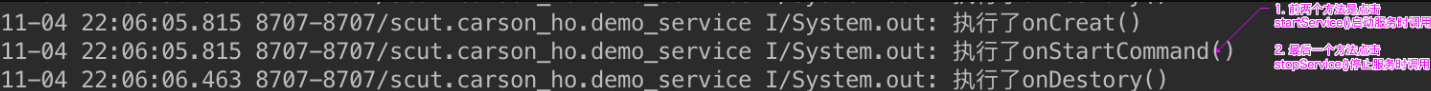
\includegraphics[width=.9\linewidth]{./pic/log.png}
\item Demo地址
\label{sec-3-4-1-4}
\begin{itemize}
\item Carson.ho的Github地址:Demo\_for\_Service
\begin{itemize}
\item \url{https://github.com/Carson-Ho/Demo_Service/tree/5e2a70cf2d75c56bbfa1abc0ead16c5ad8cae83f}
\end{itemize}
\end{itemize}
\end{enumerate}
\subsubsection{可通信的服务Service}
\label{sec-3-4-2}
\begin{itemize}
\item 上面介绍的Service是最基础的,但只能单机使用,即无法与Activity通信
\item 接下来将在上面的基础用法上,增设"与Activity通信”的功能,即使用绑定Service服务(Binder类、bindService()、onBind()、unbindService()、onUnbind())
\end{itemize}
\begin{enumerate}
\item 实例Demo
\label{sec-3-4-2-1}
接下来我将用一个实例Demo进行可通信的服务Service说明
\begin{itemize}
\item 建议先下载Demo再进行阅读:(carson.ho的Github地址)Demo\_for\_Service
\begin{itemize}
\item \url{https://github.com/Carson-Ho/Demo_Service/tree/719e3b9ffd5017c334cdfdaf45b6a72776a2066a}
\end{itemize}
\item 步骤1:在新建子类继承Service类,并新建一个子类继承自Binder类、写入与Activity关联需要的方法、创建实例
\begin{minted}[frame=lines,fontsize=\scriptsize,linenos=false]{java}
public class MyService extends Service {
    private MyBinder mBinder = new MyBinder();
    @Override
    public void onCreate() {
        super.onCreate();
        System.out.println("执行了onCreat()");
    }
    @Override
    public int onStartCommand(Intent intent, int flags, int startId) {
        System.out.println("执行了onStartCommand()");
        return super.onStartCommand(intent, flags, startId);
    }
    @Override
    public void onDestroy() {
        super.onDestroy();
        System.out.println("执行了onDestory()");
    }
    @Nullable
    @Override
    public IBinder onBind(Intent intent) {
        System.out.println("执行了onBind()");
        //返回实例
        return mBinder;
    }
    @Override
    public boolean onUnbind(Intent intent) {
        System.out.println("执行了onUnbind()");
        return super.onUnbind(intent);
    }
    //新建一个子类继承自Binder类
    class MyBinder extends Binder {
        public void service_connect_Activity() {
            System.out.println("Service关联了Activity,并在Activity执行了Service的方法");
        }
    }
}
\end{minted}
\item 步骤2:在主布局文件再设置两个Button分别用于绑定和解绑Service
\begin{minted}[frame=lines,fontsize=\scriptsize,linenos=false]{xml}
<?xml version="1.0" encoding="utf-8"?>
<RelativeLayout xmlns:android="http://schemas.android.com/apk/res/android"
    xmlns:tools="http://schemas.android.com/tools"
    android:layout_width="match_parent"
    android:layout_height="match_parent"
    android:paddingBottom="@dimen/activity_vertical_margin"
    android:paddingLeft="@dimen/activity_horizontal_margin"
    android:paddingRight="@dimen/activity_horizontal_margin"
    android:paddingTop="@dimen/activity_vertical_margin"
    tools:context="scut.carson_ho.demo_service.MainActivity">
    <Button
        android:layout_centerInParent="true"
        android:id="@+id/startService"
        android:layout_width="wrap_content"
        android:layout_height="wrap_content"
        android:text="启动服务" />
    <Button
        android:layout_centerInParent="true"
        android:layout_below="@+id/startService"
        android:id="@+id/stopService"
        android:layout_width="wrap_content"
        android:layout_height="wrap_content"
        android:text="停止服务" />
    <Button
        android:layout_centerInParent="true"
        android:layout_below="@id/stopService"
        android:id="@+id/bindService"
        android:layout_width="wrap_content"
        android:layout_height="wrap_content"
        android:text="绑定服务" />
    <Button
        android:layout_centerInParent="true"
        android:layout_below="@id/bindService"
        android:id="@+id/unbindService"
        android:layout_width="wrap_content"
        android:layout_height="wrap_content"
        android:text="解绑服务"
        />
</RelativeLayout>
\end{minted}
\item 步骤3:在Activity通过调用MyBinder类中的public方法来实现Activity与Service的联系
\begin{itemize}
\item 即实现了Activity指挥Service干什么Service就去干什么的功能
\item MainActivity.java
\end{itemize}
\begin{minted}[frame=lines,fontsize=\scriptsize,linenos=false]{java}
public class MainActivity extends AppCompatActivity implements View.OnClickListener {
    private Button startService;
    private Button stopService;
    private Button bindService;
    private Button unbindService;
    private MyService.MyBinder myBinder;
    
    // 创建ServiceConnection的匿名类
    private ServiceConnection connection = new ServiceConnection() {
            // 重写onServiceConnected()方法和onServiceDisconnected()方法
            // 在Activity与Service建立关联和解除关联的时候调用
            @Override
            public void onServiceDisconnected(ComponentName name) {
            }
            // 在Activity与Service解除关联的时候调用
            @Override
            public void onServiceConnected(ComponentName name, IBinder service) {
                // 实例化Service的内部类myBinder
                // 通过向下转型得到了MyBinder的实例
                myBinder = (MyService.MyBinder) service;
                // 在Activity调用Service类的方法
                myBinder.service_connect_Activity();
            }
        };
    @Override
    protected void onCreate(Bundle savedInstanceState) {
        super.onCreate(savedInstanceState);
        setContentView(R.layout.activity_main);
        startService = (Button) findViewById(R.id.startService);
        stopService = (Button) findViewById(R.id.stopService);
        startService.setOnClickListener(this);
        stopService.setOnClickListener(this);
        bindService = (Button) findViewById(R.id.bindService);
        unbindService = (Button) findViewById(R.id.unbindService);
        bindService.setOnClickListener(this);
        unbindService.setOnClickListener(this);
    }
    @Override
    public void onClick(View v) {
        switch (v.getId()) {
            // 点击启动Service
        case R.id.startService:
            // 构建启动服务的Intent对象
            Intent startIntent = new Intent(this, MyService.class);
            // 调用startService()方法-传入Intent对象,以此启动服务
            startService(startIntent);
            break;
            // 点击停止Service
        case R.id.stopService:
            // 构建停止服务的Intent对象
            Intent stopIntent = new Intent(this, MyService.class);
            // 调用stopService()方法-传入Intent对象,以此停止服务
            stopService(stopIntent);
            break;
            // 点击绑定Service
        case R.id.bindService:
            // 构建绑定服务的Intent对象
            Intent bindIntent = new Intent(this, MyService.class);
            // 调用bindService()方法,以此停止服务
            bindService(bindIntent,connection,BIND_AUTO_CREATE);
            // 参数说明
            // 第一个参数:Intent对象
            // 第二个参数:上面创建的Serviceconnection实例
            // 第三个参数:标志位
            // 这里传入BIND_AUTO_CREATE表示在Activity和Service建立关联后自动创建Service
            // 这会使得MyService中的onCreate()方法得到执行,但onStartCommand()方法不会执行
            break;
            // 点击解绑Service
        case R.id.unbindService:
            // 调用unbindService()解绑服务
            // 参数是上面创建的Serviceconnection实例
            unbindService(connection);
            break;
        default:
            break;
        }
    }
}
\end{minted}
\end{itemize}

\item 测试结果
\label{sec-3-4-2-2}

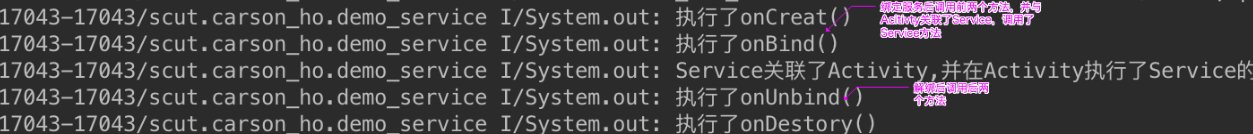
\includegraphics[width=.9\linewidth]{./pic/log2.png}
\item Demo
\label{sec-3-4-2-3}
\begin{itemize}
\item carson.ho的Github地址:Demo\_for\_Service
\begin{itemize}
\item \url{https://github.com/Carson-Ho/Demo_Service/tree/719e3b9ffd5017c334cdfdaf45b6a72776a2066a}
\end{itemize}
\end{itemize}
\end{enumerate}
\subsubsection{前台Service}
\label{sec-3-4-3}
\begin{itemize}
\item 前台Service和后台Service(普通)最大的区别就在于:
\begin{itemize}
\item 前台Service在下拉通知栏有显示通知,但后台Service没有;
\item 前台Service优先级较高,不会由于系统内存不足而被回收;后台Service优先级较低,当系统出现内存不足情况时,很有可能会被回收
\end{itemize}
\end{itemize}
\begin{enumerate}
\item 具体使用
\label{sec-3-4-3-1}
\begin{itemize}
\item 用法很简单,只需要在原有的Service类对onCreate()方法进行稍微修改即可,如下图:
\begin{minted}[frame=lines,fontsize=\scriptsize,linenos=false]{java}
@Override
public void onCreate() {
    super.onCreate();
    System.out.println("执行了onCreat()");

    // 添加下列代码将后台Service变成前台Service
    // 构建"点击通知后打开MainActivity"的Intent对象
    Intent notificationIntent = new Intent(this,MainActivity.class);
    PendingIntent pendingIntent = PendingIntent.getActivity(this,0,notificationIntent,0);
    // 新建Builer对象
    Notification.Builder builer = new Notification.Builder(this);
    builer.setContentTitle("前台服务通知的标题");// 设置通知的标题
    builer.setContentText("前台服务通知的内容"); // 设置通知的内容
    builer.setSmallIcon(R.mipmap.ic_launcher); // 设置通知的图标
    builer.setContentIntent(pendingIntent);    // 设置点击通知后的操作
    Notification notification = builer.getNotification();// 将Builder对象转变成普通的notification
    startForeground(1, notification);// 让Service变成前台Service,并在系统的状态栏显示出来
}
\end{minted}
\end{itemize}
\item 测试结果
\label{sec-3-4-3-2}
\begin{itemize}
\item 运行后,当点击Start Service或Bind Service按钮,Service就会以前台Service的模式启动(通知栏上有通知),如下图

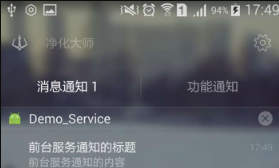
\includegraphics[width=.9\linewidth]{./pic/frontService.png}
\end{itemize}
\end{enumerate}
\subsubsection{远程Service}
\label{sec-3-4-4}
\begin{itemize}
\item 具体请看我写的另外一篇文章:Android:远程服务Service(含AIDL \& IPC讲解)
\begin{itemize}
\item \url{https://www.jianshu.com/p/34326751b2c6}
\end{itemize}
\end{itemize}
\subsection{使用场景}
\label{sec-3-5}
\begin{itemize}
\item 通过上述描述,你应该对Service类型及其使用非常了解;
\item 那么,我们该什么时候用哪种类型的Service呢?
\item 各种Service的使用场景请看下图:

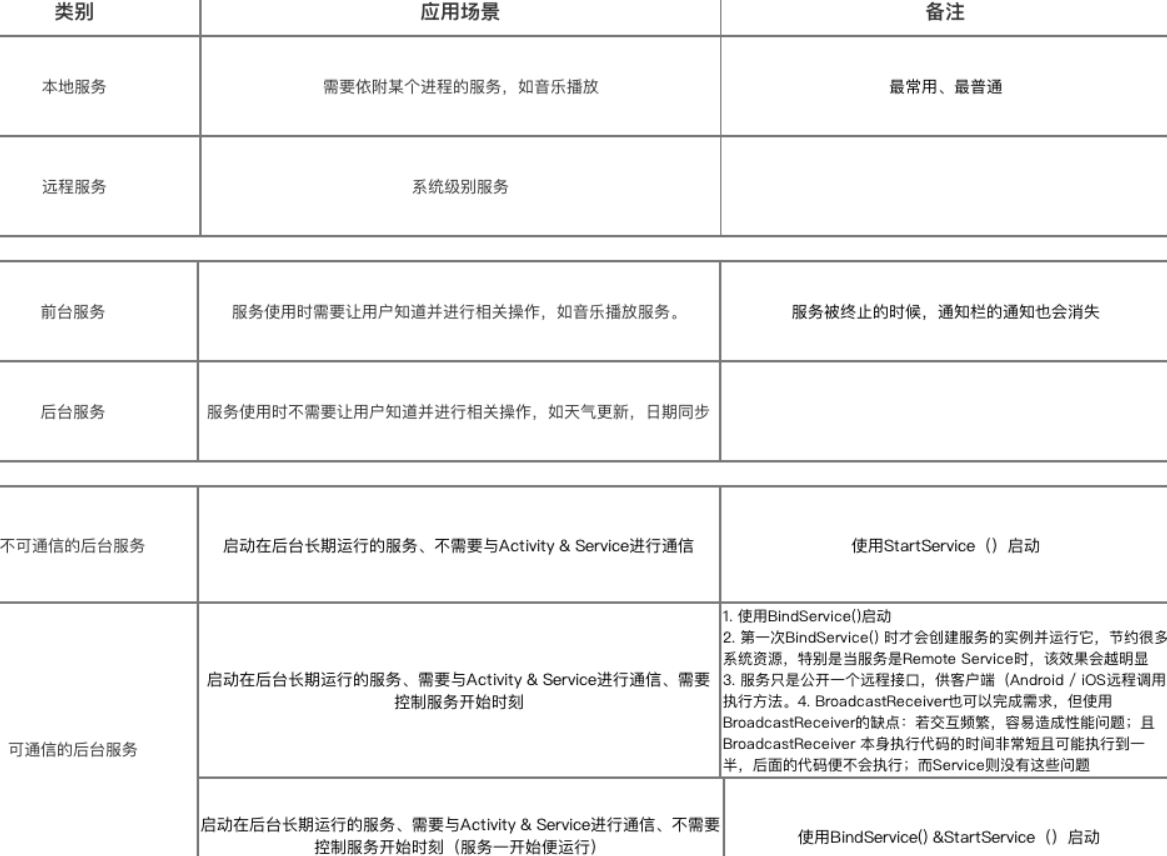
\includegraphics[width=.9\linewidth]{./pic/use.png}
\end{itemize}

\begin{center}
\begin{tabular}{lllll}
\hline
类型 & 特点 & 优点 & 缺点 & 应用场景\\
\hline
本地 & -运行在主线程 & -节约资源 & -限制性大 & -需依附某个进程的服务\\
 & -主进程被禁止后,服务也会终止 & -通信方便: & 主进程被禁止后, & (最常用的服务类型如音乐播放)\\
 &  & 因在同一进程因此不需IPC和AIDL & 服务也会终止 & \\
\hline
远程 & -运行在独立进程 & -灵活: & -消耗资源:单独进程 & -系统级别服务\\
 & -服务常驻在后台, & 服务常驻在后台, & -使用AIDL进行IPC复杂 & \\
 & 不受其它activity影响 & 不受其它activity影响 &  & \\
\hline
\end{tabular}
\end{center}

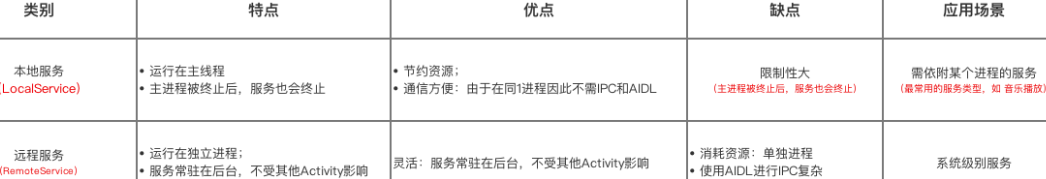
\includegraphics[width=.9\linewidth]{./pic/location.png}
\begin{itemize}
\item 按运行类型分类

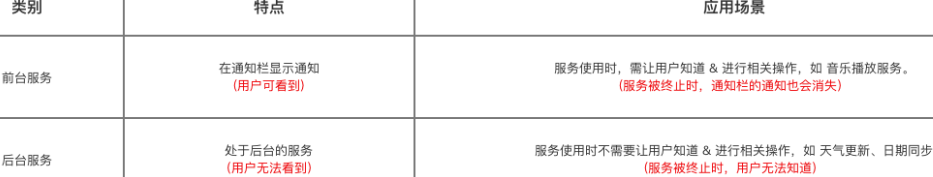
\includegraphics[width=.9\linewidth]{./pic/category.png}
\end{itemize}
\begin{center}
\begin{tabular}{llll}
\hline
类型 & 应用场景 & 备注 & \\
\hline
本地服务 & 需依附某个进程的服务,如音乐播放 & 最常用、最普通 & \\
远程服务 & 系统级别服务 &  & \\
\hline
前台服务 & 服务使用时需让用户知道并进行相关操作,如音乐播放 & 服务被终止时,通知栏的通知也会消失 & \\
后台服务 & 服务使用时不需让用户知道并进行相关操作,如天气更新、日期同步 & 服务被终止时,用户无法知道 & \\
\hline
不可通信服务 & 启动在后台长期运行的服务, & 使用startService()启动 & \\
 & \textbf{不} 需与Activity \& Service通信 &  & \\
\hline
可通信服务 & 启动在后台长期运行的服务, & 用bindService()启动 & \\
 & 需与Activity \& Service通信 & *备注 & \\
 & 需控制服务开启时刻 &  & \\
\hline
可通信服务 & 启动在后台长期运行的服务, & 使用startService()、bindService()启动 & \\
 & 需与Activity \& Service通信 &  & \\
 & \textbf{不} 需控制服务开启时刻 &  & \\
\hline
\end{tabular}
\end{center}
\begin{itemize}
\item 备注
\begin{itemize}
\item 用bindService()启动
\item 第一次bindService()时才会创建服务的实例并运行它,节约很多系统资源,特别是当服务是Remote Service时,该效果会更明显
\item 服务只是公开一个远程接口,供客户端Android、iOS远程调用执行方法
\item BroadcastReceiver也可完成需求,但使用BroadcastReceiver的缺点:若交互频繁,容易造成性能问题;且BroadcastReceiver本身执行代码的时间非常短且可能执行到一半,后面的代码便不会执行,而Service则没有这些问题
\end{itemize}
\end{itemize}

\section{Android 多线程 解析:IntentService(含源码解析)}
\label{sec-4}
\begin{itemize}
\item \url{https://www.jianshu.com/p/8a3c44a9173a}
\end{itemize}
\subsection{前言}
\label{sec-4-1}
\begin{itemize}
\item 多线程的应用在Android开发中是非常常见的,常用方法主要有:
\begin{itemize}
\item 继承Thread类
\item 实现Runnable接口
\item AsyncTask
\item Handler
\item HandlerThread
\item IntentService
\end{itemize}
\item 今天,我将全面解析多线程其中一种常见用法:IntentService
\end{itemize}
\subsection{定义}
\label{sec-4-2}
\begin{itemize}
\item Android里的一个封装类,继承四大组件之一的Service
\end{itemize}
\subsection{作用}
\label{sec-4-3}
\begin{itemize}
\item 处理异步请求 \& 实现多线程
\end{itemize}
\subsection{使用场景}
\label{sec-4-4}
\begin{itemize}
\item 线程任务 需 按顺序、在后台执行
\begin{itemize}
\item 最常见的场景:离线下载
\item 不符合多个数据同时请求的场景:所有的任务都在同一个Thread looper里执行
\end{itemize}
\end{itemize}
\subsection{使用步骤}
\label{sec-4-5}
\begin{itemize}
\item 步骤1:定义 IntentService的子类
\begin{itemize}
\item 需传入线程名称、复写onHandleIntent()方法
\end{itemize}
\item 步骤2:在Manifest.xml中注册服务
\item 步骤3:在Activity中开启Service服务
\end{itemize}
\subsection{实例应用}
\label{sec-4-6}
\begin{itemize}
\item 步骤1:定义 IntentService的子类
\begin{itemize}
\item 传入线程名称、复写onHandleIntent()方法
\end{itemize}
\begin{minted}[frame=lines,fontsize=\scriptsize,linenos=false]{java}
public class myIntentService extends IntentService {
    // 在构造函数中传入线程名字
    public myIntentService() {
        // 调用父类的构造函数
        // 参数 = 工作线程的名字
        super("myIntentService");
    }
   /** 
     * 复写onHandleIntent()方法
     * 根据 Intent实现 耗时任务 操作
     **/  
    @Override
    protected void onHandleIntent(Intent intent) {
        // 根据 Intent的不同,进行不同的事务处理
        String taskName = intent.getExtras().getString("taskName");
        switch (taskName) {
            case "task1":
                Log.i("myIntentService", "do task1");
                break;
            case "task2":
                Log.i("myIntentService", "do task2");
                break;
            default:
                break;
        }
    }
    @Override
    public void onCreate() {
        Log.i("myIntentService", "onCreate");
        super.onCreate();
    }
   /** 
     * 复写onStartCommand()方法
     * 默认实现 = 将请求的Intent添加到工作队列里
     **/  
    @Override
    public int onStartCommand(Intent intent, int flags, int startId) {
        Log.i("myIntentService", "onStartCommand");
        return super.onStartCommand(intent, flags, startId);
    }
    @Override
    public void onDestroy() {
        Log.i("myIntentService", "onDestroy");
        super.onDestroy();
    }
}
\end{minted}
\item 步骤2:在Manifest.xml中注册服务
\begin{minted}[frame=lines,fontsize=\scriptsize,linenos=false]{xml}
<service android:name=".myIntentService">
            <intent-filter >
                <action android:name="cn.scu.finch"/>
            </intent-filter>
        </service>
\end{minted}
\item 步骤3:在Activity中开启Service服务
\begin{minted}[frame=lines,fontsize=\scriptsize,linenos=false]{java}
public class MainActivity extends AppCompatActivity {
    @Override
    protected void onCreate(Bundle savedInstanceState) {
        super.onCreate(savedInstanceState);
        setContentView(R.layout.activity_main);
        // 同一服务只会开启1个工作线程
        // 在onHandleIntent()函数里,依次处理传入的Intent请求
        // 将请求通过Bundle对象传入到Intent,再传入到服务里
        // 请求1
        Intent i = new Intent("cn.scu.finch");
        Bundle bundle = new Bundle();
        bundle.putString("taskName", "task1");
        i.putExtras(bundle);
        startService(i);
        // 请求2
        Intent i2 = new Intent("cn.scu.finch");
        Bundle bundle2 = new Bundle();
        bundle2.putString("taskName", "task2");
        i2.putExtras(bundle2);
        startService(i2);
        startService(i);  //多次启动
    }
}
\end{minted}
\item 测试结果
\begin{minted}[frame=lines,fontsize=\scriptsize,linenos=false]{java}
Tag Text
myIntentService onCreate
myIntentService onStartCommand
myIntentService onStartCommand
myIntentService do task1
myIntentService onStartCommand
myIntentService do task2
myIntentService do task1
myIntentService onDestory
\end{minted}
\end{itemize}

\subsection{源码分析}
\label{sec-4-7}
\begin{itemize}
\item IntentService的源码工作流程如下:

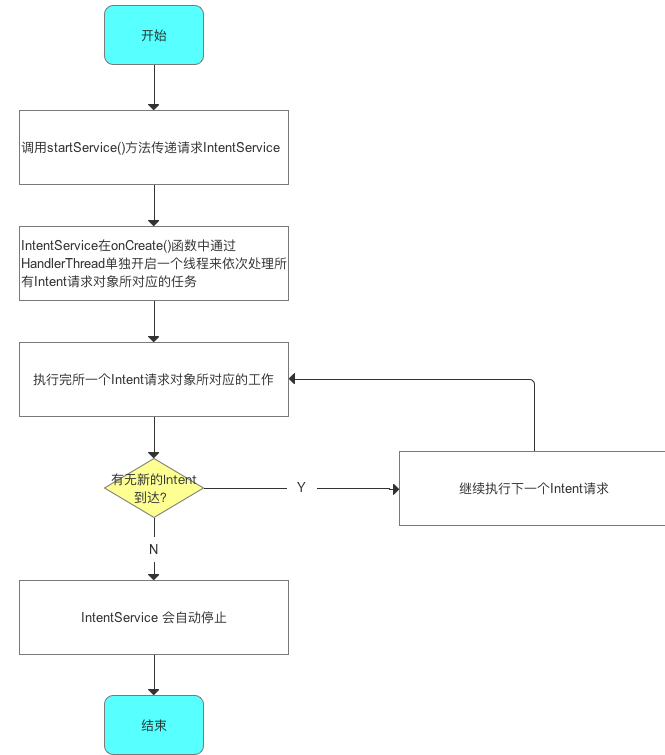
\includegraphics[width=.9\linewidth]{./pic/IntentService.png}
\item 特别注意:若启动IntentService 多次,那么 每个耗时操作 则 以队列的方式 在 IntentService的 onHandleIntent回调方法中依次执行,执行完自动结束
\item 接下来,我们将通过 源码分析 解决以下问题:
\begin{itemize}
\item IntentService 如何单独开启1个新的工作线程
\item IntentService 如何通过onStartCommand() 将Intent 传递给服务 \& 依次插入到工作队列中
\end{itemize}
\end{itemize}
\subsubsection{IntentService如何单独开启1个新的工作线程}
\label{sec-4-7-1}
\begin{itemize}
\item 主要分析内容  = IntentService源码中的 onCreate()方法
\begin{minted}[frame=lines,fontsize=\scriptsize,linenos=false]{java}
@Override
public void onCreate() {
    super.onCreate();
    
    // 1. 通过实例化andlerThread新建线程 & 启动;故 使用IntentService时,不需额外新建线程
    // HandlerThread继承自Thread,内部封装了 Looper
    HandlerThread thread = new HandlerThread("IntentService[" + mName + "]");
    thread.start();
  
    // 2. 获得工作线程的 Looper & 维护自己的工作队列
    mServiceLooper = thread.getLooper();
    // 3. 新建mServiceHandler & 绑定上述获得Looper
    // 新建的Handler 属于工作线程 ->>分析1
    mServiceHandler = new ServiceHandler(mServiceLooper); 
}
/** 
 * 分析1:ServiceHandler源码分析
 **/ 
 private final class ServiceHandler extends Handler {
     // 构造函数
     public ServiceHandler(Looper looper) {
     super(looper);
   }
    // IntentService的handleMessage()把接收的消息交给onHandleIntent()处理
    @Override
     public void handleMessage(Message msg) {

      // onHandleIntent 方法在工作线程中执行
      // onHandleIntent() = 抽象方法,使用时需重写 ->>分析2
      onHandleIntent((Intent)msg.obj);
      // 执行完调用 stopSelf() 结束服务
      stopSelf(msg.arg1);
    }
}
/** 
 * 分析2: onHandleIntent()源码分析
 * onHandleIntent() = 抽象方法,使用时需重写
 **/ 
@WorkerThread
protected abstract void onHandleIntent(Intent intent);
\end{minted}
\end{itemize}
\subsubsection{IntentService 如何通过onStartCommand() 将Intent 传递给服务 \& 依次插入到工作队列中}
\label{sec-4-7-2}
\begin{minted}[frame=lines,fontsize=\scriptsize,linenos=false]{java}
/** 
 * onStartCommand()源码分析
 * onHandleIntent() = 抽象方法,使用时需重写
 **/ 
public int onStartCommand(Intent intent, int flags, int startId) {
    // 调用onStart()->>分析1
    onStart(intent, startId);
    return mRedelivery ? START_REDELIVER_INTENT : START_NOT_STICKY;
}
/** 
  * 分析1:onStart(intent, startId)
  **/ 
  public void onStart(Intent intent, int startId) {
    // 1. 获得ServiceHandler消息的引用
    Message msg = mServiceHandler.obtainMessage();
    msg.arg1 = startId;
    // 2. 把 Intent参数 包装到 message 的 obj 发送消息中,
    //这里的Intent  = 启动服务时startService(Intent) 里传入的 Intent
    msg.obj = intent;
    // 3. 发送消息,即 添加到消息队列里
    mServiceHandler.sendMessage(msg);
}
\end{minted}
\subsection{总结}
\label{sec-4-8}
从上面源码可看出:IntentService本质 = Handler + HandlerThread:
\begin{itemize}
\item 通过HandlerThread 单独开启1个工作线程:IntentService
\item 创建1个内部 Handler :ServiceHandler
\item 绑定 ServiceHandler 与 IntentService
\item 通过 onStartCommand() 传递服务intent 到ServiceHandler、依次插入Intent到工作队列中 \& 逐个发送给 onHandleIntent()
\item 通过onHandleIntent()依次处理所有Intent对象所对应的任务
\begin{itemize}
\item 因此我们通过复写onHandleIntent() \& 在里面 根据Intent的不同进行不同线程操作 即可
\end{itemize}
\end{itemize}

\subsection{注意事项}
\label{sec-4-9}
\begin{enumerate}
\item 工作任务队列 = 顺序执行
\label{sec-4-9-0-1}

即 若一个任务正在IntentService中执行,此时你再发送1个新的任务请求,这个新的任务会一直等待直到前面一个任务执行完毕后才开始执行
\begin{itemize}
\item 原因:
\begin{itemize}
\item 由于onCreate()只会调用一次 = 只会创建1个工作线程;
\item 当多次调用 startService(Intent)时(即 onStartCommand()也会调用多次),其实不会创建新的工作线程,只是把消息加入消息队列中 \& 等待执行。
\item 所以,多次启动 IntentService 会按顺序执行事件
\end{itemize}
\end{itemize}

若服务停止,则会清除消息队列中的消息,后续的事件不执行
\item 不建议通过 bindService() 启动 IntentService
\label{sec-4-9-0-2}

原因:
\begin{minted}[frame=lines,fontsize=\scriptsize,linenos=false]{java}
// 在IntentService中,onBind()`默认返回null
@Override
public IBinder onBind(Intent intent) {
    return null;
}
\end{minted}
\begin{itemize}
\item 采用 bindService()启动 IntentService的生命周期如下:
\begin{minted}[frame=lines,fontsize=\scriptsize,linenos=false]{java}
onCreate() ->> onBind() ->> onUnbind()->> onDestory()
\end{minted}
\item 即,并不会调用onStart() 或 onStartcommand(),故不会将消息发送到消息队列,那么onHandleIntent()将不会回调,即无法实现多线程的操作
\begin{itemize}
\item 此时,你应该使用Service,而不是IntentService
\end{itemize}
\end{itemize}
\end{enumerate}
\subsection{对比}
\label{sec-4-10}
\subsubsection{IntentService与Service的区别}
\label{sec-4-10-1}
\begin{center}
\begin{tabular}{lll}
\hline
类型 & 运行线程 & 结束服务操作\\
\hline
Service & 主线程 & 需主动调用stopService()\\
 & 不能处理耗时操作,否则会出现ANR & \\
\hline
IntentService & 创建一个工作线程处理多线程任务 & 不需要\\
 &  & 在所有Intent被处理完后系统会自动关闭服务\\
\hline
\end{tabular}
\end{center}

\begin{itemize}
\item 备注:
\begin{itemize}
\item IntentService为Service的onBind()提供了默认实现:返回null
\item IntentService为Service的onStartCommand()提供了默认实现:将请求的intent添加到队列中
\end{itemize}
\end{itemize}
\subsubsection{IntentService与其他线程的区别}
\label{sec-4-10-2}

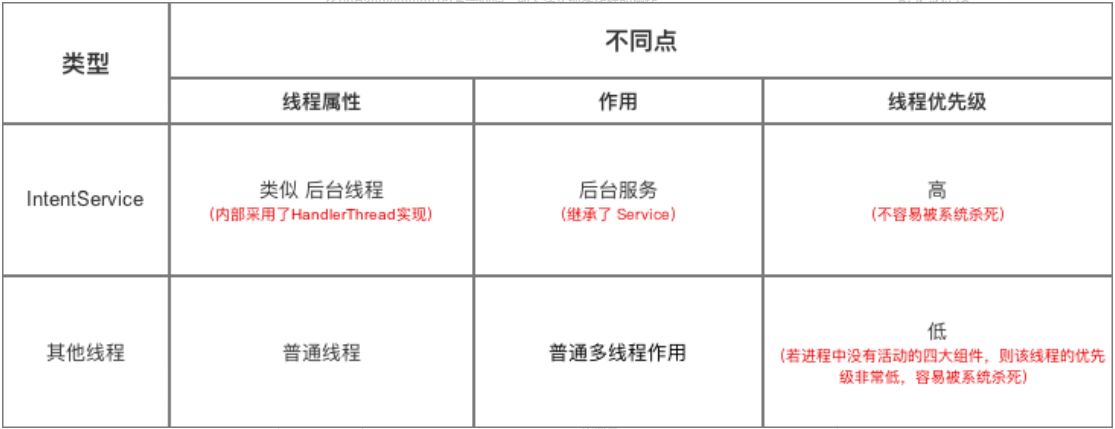
\includegraphics[width=.9\linewidth]{./pic/serviceIntentService.png}

\subsection{总结}
\label{sec-4-11}
\begin{itemize}
\item 本文主要 全面介绍了 多线程IntentService用法 \& 源码
\item 接下来,我会继续讲解Android开发中关于多线程的知识,包括继承Thread类、实现Runnable接口、Handler等等,有兴趣可以继续关注Carson\_Ho的安卓开发笔记
\end{itemize}

\section{Android:远程服务Service(含AIDL \& IPC讲解)}
\label{sec-5}
\begin{itemize}
\item \url{https://www.jianshu.com/p/34326751b2c6}
\end{itemize}
\subsection{前言}
\label{sec-5-1}
\begin{itemize}
\item Service作为Android四大组件之一,应用非常广泛
\item 本文将介绍Service其中一种常见用法:远程Service
\end{itemize}
\subsection{远程服务与本地服务的区别}
\label{sec-5-2}
\begin{itemize}
\item 远程服务与本地服务最大的区别是:远程Service与调用者不在同一个进程里(即远程Service是运行在另外一个进程);而本地服务则是与调用者运行在同一个进程里
\item 二者区别的详细区别如下图:

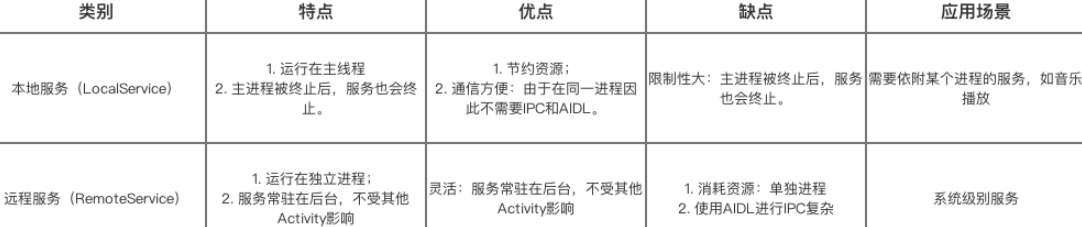
\includegraphics[width=.9\linewidth]{./pic/diff2.png}
\end{itemize}
\begin{center}
\begin{tabular}{lllll}
\hline
类型 & 特点 & 优点 & 缺点 & 应用场景\\
\hline
本地 & 1运行在主线程 & 1节约资源 & 限制性大: & 需依附某个进程的服务\\
Local & 2主进程被禁止后, & 2通信方便: & 主进程被禁止后, & (如音乐播放)\\
Service & 服务也会终止 & 在同一进程=>不需IPC和AIDL & 服务也会终止 & \\
\hline
远程 & 1运行在独立进程 & 灵活: & 1消耗资源:单独进程 & 系统级别服务\\
Remote & 2服务常驻在后台, & 服务常驻在后台, & 2使用AIDL进行IPC复杂 & \\
Service & 不受其它activity影响 & 不受其它activity影响 &  & \\
\hline
\end{tabular}
\end{center}

\subsection{使用场景}
\label{sec-5-3}
\begin{itemize}
\item 多个应用程序共享同一个后台服务(远程服务)
\begin{itemize}
\item 即一个远程Service与多个应用程序的组件(四大组件)进行跨进程通信
\end{itemize}
\end{itemize}
\subsection{使用场景}
\label{sec-5-4}

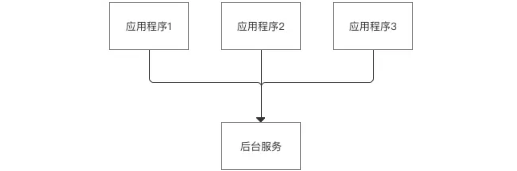
\includegraphics[width=.9\linewidth]{./pic/remoteService.png}
\subsection{具体使用}
\label{sec-5-5}
\begin{itemize}
\item 为了让远程Service与多个应用程序的组件(四大组件)进行跨进程通信(IPC),需要使用AIDL
\begin{itemize}
\item \textbf{IPC} : \textbf{Inter-Process Communication} ,即跨进程通信
\item \textbf{AIDL} : \textbf{Android Interface Definition Language} ,即Android接口定义语言;
\begin{itemize}
\item 用于让某个Service与多个应用程序组件之间进行跨进程通信,从而可以实现多个应用程序共享同一个Service的功能。
\end{itemize}
\end{itemize}
\item 在多进程通信中,存在两个进程角色(以最简单的为例):服务器端和客户端
\item 以下是两个进程角色的具体使用步骤:
\begin{itemize}
\item \textbf{服务器端(Service)}
\begin{itemize}
\item 步骤1:新建定义AIDL文件,并声明该服务需要向客户端提供的接口
\item 步骤2:在Service子类中实现AIDL中定义的接口方法,并定义生命周期的方法(onCreate()、onStartCommand()、onBind()、onUnbind()、onDestory())
\item 步骤3:在AndroidMainfest.xml中注册服务 \& 声明为远程服务
\end{itemize}
\item \textbf{客户端(Client)}
\begin{itemize}
\item 步骤1:拷贝服务端的AIDL文件到目录下
\item 步骤2:使用Stub.asInterface接口获取服务器的Binder,根据需要调用服务提供的接口方法
\item 步骤3:通过Intent指定服务端的服务名称和所在包,绑定远程Service
\end{itemize}
\end{itemize}
\item 接下来,我将用一个具体实例来介绍远程Service的使用
\end{itemize}

\subsection{具体实例}
\label{sec-5-6}
\begin{itemize}
\item 实例描述:客户端远程调用服务器端的远程Service
\item 具体使用:
\end{itemize}
\subsubsection{服务器端(Service)}
\label{sec-5-6-1}

新建一个服务器端的工程:Service - server
\begin{itemize}
\item 先下Demo再看,效果会更好:Github\_RemoteService\_Server
\item 步骤1. 新建一个AIDL文件
\begin{itemize}
\item New ==> AIDL ==> AIDL File
\end{itemize}
\item 步骤2. 在新建AIDL文件里定义Service需要与Activity进行通信的内容(方法),并进行编译(Make Project)
\begin{minted}[frame=lines,fontsize=\scriptsize,linenos=false]{java}
// 在新建的AIDL_Service1.aidl里声明需要与Activity进行通信的方法
package scut.carson_ho.demo_service;
interface AIDL_Service1 {
    void AIDL_Service();
}
//AIDL中支持以下的数据类型
//1. 基本数据类型
//2. String 和CharSequence
//3. List 和 Map ,List和Map 对象的元素必须是AIDL支持的数据类型;
//4. AIDL自动生成的接口(需要导入-import)
//5. 实现android.os.Parcelable 接口的类(需要导入-import)
\end{minted}
\end{itemize}

编译
\begin{itemize}
\item 步骤3:在Service子类中实现AIDL中定义的接口方法,并定义生命周期的方法(onCreate()、onBind()、onUnbind() etc)
\begin{itemize}
\item MyService.java
\end{itemize}
\begin{minted}[frame=lines,fontsize=\scriptsize,linenos=false]{java}
/** 
 * onStartCommand()源码分析
 * onHandleIntent() = 抽象方法,使用时需重写
 **/ 
public int onStartCommand(Intent intent, int flags, int startId) {
    // 调用onStart()->>分析1
    onStart(intent, startId);
    return mRedelivery ? START_REDELIVER_INTENT : START_NOT_STICKY;
}
/** 
 * 分析1:onStart(intent, startId)
 **/ 
public void onStart(Intent intent, int startId) {
    // 1. 获得ServiceHandler消息的引用
    Message msg = mServiceHandler.obtainMessage();
    msg.arg1 = startId;
    // 2. 把 Intent参数 包装到 message 的 obj 发送消息中,
    //这里的Intent  = 启动服务时startService(Intent) 里传入的 Intent
    msg.obj = intent;
    // 3. 发送消息,即 添加到消息队列里
    mServiceHandler.sendMessage(msg);
}
\end{minted}
\item 步骤4:在AndroidMainfest.xml中注册服务 \& 声明为远程服务
\begin{minted}[frame=lines,fontsize=\scriptsize,linenos=false]{xml}
<service
    android:name=".MyService"
    android:process=":remote"  //将本地服务设置成远程服务
    android:exported="true"      //设置可被其他进程调用
    //该Service可以响应带有scut.carson_ho.service_server.AIDL_Service1这个action的Intent。
    //此处Intent的action必须写成"服务器端包名.aidl文件名”
    <intent-filter>
      <action android:name="scut.carson_ho.service_server.AIDL_Service1"/>
    </intent-filter>
</service>
\end{minted}
\item 至此,服务器端(远程Service)已经完成了。
\end{itemize}
\subsubsection{客户端(Client)}
\label{sec-5-6-2}

新建一个客户端的工程:Service - Client
\begin{itemize}
\item 先下Demo再看,效果会更好:Github\_RemoteService\_Client
\item 步骤1:将服务端的AIDL文件所在的包复制到客户端目录下(Project/app/src/main),并进行编译
\begin{itemize}
\item 注:记得要原封不动地复制!!什么都不要改!
\end{itemize}
\item 步骤2:在主布局文件定义"绑定服务”的按钮
\begin{itemize}
\item MainActivity.xml
\end{itemize}
\begin{minted}[frame=lines,fontsize=\scriptsize,linenos=false]{xml}
<?xml version="1.0" encoding="utf-8"?>
<RelativeLayout xmlns:android="http://schemas.android.com/apk/res/android"
    xmlns:tools="http://schemas.android.com/tools"
    android:layout_width="match_parent"
    android:layout_height="match_parent"
    android:paddingBottom="@dimen/activity_vertical_margin"
    android:paddingLeft="@dimen/activity_horizontal_margin"
    android:paddingRight="@dimen/activity_horizontal_margin"
    android:paddingTop="@dimen/activity_vertical_margin"
    tools:context="scut.carson_ho.service_client.MainActivity">
    <Button
        android:layout_centerInParent="true"
        android:id="@+id/bind_service"
        android:layout_width="match_parent"
        android:layout_height="wrap_content"
        android:text="绑定服务"
        />
</RelativeLayout>
\end{minted}
\item 步骤3:在MainActivity.java里
\begin{itemize}
\item 使用Stub.asInterface接口获取服务器的Binder;
\item 通过Intent指定服务端的服务名称和所在包,进行Service绑定;
\item 根据需要调用服务提供的接口方法。
\item MainActivity.java
\end{itemize}
\begin{minted}[frame=lines,fontsize=\scriptsize,linenos=false]{java}
public class MainActivity extends AppCompatActivity {
    private Button bindService;
    // 定义aidl接口变量
    private AIDL_Service1 mAIDL_Service;
    // 创建ServiceConnection的匿名类
    private ServiceConnection connection = new ServiceConnection() {
        // 重写onServiceConnected()方法和onServiceDisconnected()方法
        // 在Activity与Service建立关联和解除关联的时候调用
        @Override
        public void onServiceDisconnected(ComponentName name) {
        }
        // 在Activity与Service建立关联时调用
        @Override
        public void onServiceConnected(ComponentName name, IBinder service) {
            // 使用AIDLService1.Stub.asInterface()方法获取服务器端返回的IBinder对象
            // 将IBinder对象传换成了mAIDL_Service接口对象
            mAIDL_Service = AIDL_Service1.Stub.asInterface(service);
            try {
                // 通过该对象调用在MyAIDLService.aidl文件中定义的接口方法,从而实现跨进程通信
                mAIDL_Service.AIDL_Service();
            } catch (RemoteException e) {
                e.printStackTrace();
            }
        }
    };

    @Override
    protected void onCreate(Bundle savedInstanceState) {
        super.onCreate(savedInstanceState);
        setContentView(R.layout.activity_main);
        bindService = (Button) findViewById(R.id.bind_service);
        // 设置绑定服务的按钮
        bindService.setOnClickListener(new View.OnClickListener() {
            @Override
            public void onClick(View v) {

                // 通过Intent指定服务端的服务名称和所在包,与远程Service进行绑定
                // 参数与服务器端的action要一致,即"服务器包名.aidl接口文件名"
                Intent intent = new Intent("scut.carson_ho.service_server.AIDL_Service1");

                // Android5.0后无法只通过隐式Intent绑定远程Service
                // 需要通过setPackage()方法指定包名
                intent.setPackage("scut.carson_ho.service_server");

                // 绑定服务,传入intent和ServiceConnection对象
                bindService(intent, connection, Context.BIND_AUTO_CREATE);
            }
        });
    }
}
\end{minted}
\end{itemize}
\subsubsection{测试结果}
\label{sec-5-6-3}

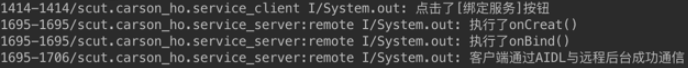
\includegraphics[width=.9\linewidth]{./pic/serverClient.png}
\begin{itemize}
\item 从上面测试结果可以看出:
\begin{itemize}
\item 打印的语句分别运行在不同进程(看语句前面的包名);
\item 客户端调用了服务端Service的方法
\end{itemize}
\item 即客户端和服务端进行了跨进程通信
\end{itemize}
\subsubsection{Demo地址}
\label{sec-5-6-4}
\begin{itemize}
\item 客户端:Github\_RemoteService\_Client
\item 服务端:Github\_RemoteService\_Server
\end{itemize}
% Emacs 27.1 (Org mode 8.2.7c)
\end{document}